\documentclass[tikz,transparent]{standalone}

\usepackage{amsmath, amssymb}

\usetikzlibrary{positioning,automata,calc}

\begin{document}

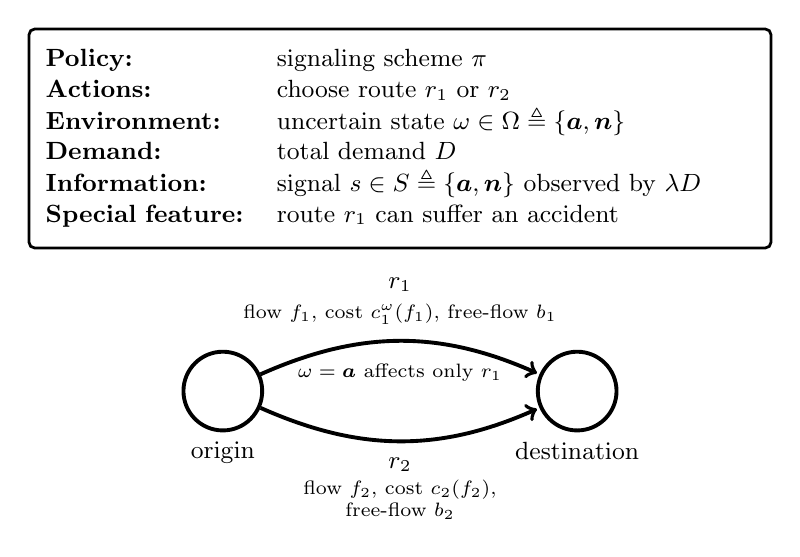
\begin{tikzpicture}[
    font=\small,
    shorten >=1pt,
    node distance=2cm,
    on grid,
    auto,
    every state/.style={
        draw,
        circle,
        line width=1.4pt,
        minimum size=10mm,
        inner sep=0pt
    },
    route/.style={
        draw,
        ->,
        line width=1.4pt
    },
    panel/.style={
        draw,
        rounded corners=2pt,
        line width=1pt,
        align=left,
        inner sep=6pt,
        text width=9cm
    }
]
    % nodes
    \node[state,label=below:{origin}] (q_0) {};
    \node[state,label=below:{destination}] (q_1) [right=4.5cm of q_0] {};

    % midpoint for top panel
    \coordinate (mid) at ($(q_0)!0.5!(q_1)$);

    % top information panel
    \node[panel,above=1.8cm of mid] (info) {
        \begin{tabular}{@{}ll@{}}
        \textbf{Policy:} & signaling scheme $\pi$ \\
        \textbf{Actions:} & choose route $r_1$ or $r_2$ \\
        \textbf{Environment:} & uncertain state $\omega\in\Omega\triangleq\{\boldsymbol{a},\boldsymbol{n}\}$ \\
        \textbf{Demand:} & total demand $D$ \\
        \textbf{Information:} & signal $s\in S\triangleq\{\boldsymbol{a},\boldsymbol{n}\}$ observed by $\lambda D$ \\
        \textbf{Special feature:} & route $r_1$ can suffer an accident
        \end{tabular}
    };

    % routes
    \path[route]
        (q_0) edge[bend left=24]
            node[pos=0.5,above=14pt,align=center] {$r_1$}
            node[pos=0.5,above=2pt,align=center,font=\scriptsize] {flow $f_1$, cost $c_1^\omega(f_1)$, free-flow $b_1$}
            (q_1)
        (q_0) edge[bend right=24]
            node[pos=0.5,below=2pt,align=center] {$r_2$}
            node[pos=0.5,below=10pt,align=center,font=\scriptsize] {flow $f_2$, cost $c_2(f_2)$,\\free-flow $b_2$}
            (q_1);

    \node[font=\scriptsize,above=0pt of mid] {$\omega=\boldsymbol{a}$ affects only $r_1$};
\end{tikzpicture}

\end{document}
